\scanpage{5}

\diagram{\begin{tikzcd}[ampersand replacement=\&,column sep=1.4em]
{\mathbb Z[\mathbb F_{\unsure{n-1|n-2|n\,2}}]}
 \& {\mathbb Z[\mathbb F_{n-1}]}\arrow[l]
 \& {\mathbb Z[F_n]}\arrow[l,"{t_n-s_n}"]
 \& {\mathbb Z[\mathbb F_{n+1}]}\arrow[l]
 \& {\begin{tikzpicture}[baseline=-.3ex,x=.5em,y=.5em,line width=.8pt]
 \draw (0,.15)--(.65,.15);\draw (.43,.55)--(.43,-.3)--(.7,-.3);
 \draw (0,0)--(0,.3);
 \end{tikzpicture}}
\end{tikzcd}}
% Detached cross-like ink after the chain; no algebraic function assigned.
\figure{\begin{tikzpicture}[x=1em,y=1em,line width=.4pt]
\draw (0,.2)--(.13,0)--(.3,-.1);
\draw (.67,.05)--(.79,.13);
\end{tikzpicture}}
% Two short separated ink strokes below and to the right of the chain.

\[
\begin{aligned}
D_n&\longrightarrow X &\quad&\deleted{D_n}\mathord{\raisebox{1ex}{\(\cdot\)}}\\
\bigl\{x&\in F_n && =
\end{aligned}
\]
% The upper trial has unmatched parentheses in the ink. No opening parenthesis
% is supplied before the first or last y-like argument.
\[
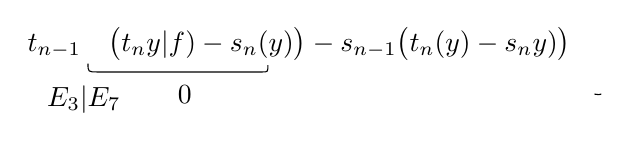
\begin{tikzpicture}[baseline=(trial.base),x=1em,y=1em,line width=.4pt]
\node[anchor=west,inner sep=0pt] (trial) at (0,0)
 {$t_{n-1}\quad\bigl(t_n\unsure{y|f})-s_n(y)\bigr)-s_{n-1}\bigl(t_n(y)-s_n y)\bigr)$};
\draw (2.2,-.7)..controls(2.2,-1)and(2.2,-1)..(2.55,-1)
 --(8.5,-1)..controls(8.7,-1)and(8.7,-1)..(8.7,-.75);
\node at (5.7,-1.8) {$0$};
\node at (2.05,-2) {$\unsure{E_3|E_7}$};
\draw (20.5,-1.8)--(20.65,-1.82)--(20.75,-1.8);
\end{tikzpicture}
\]
% The low bracket ends under the first difference, before its final closures.
% The short isolated stroke at the far right is traced without interpretation.

\[
\begin{array}{cc}
\underset{\smile}{F}_0 & F_1\\[.6em]
F'_0 & \mathbb F'_1\\
\unsure{1|\prime}&
\end{array}
\]
\diagram{\begin{tikzcd}[ampersand replacement=\&,column sep=1.7em,row sep=1.3ex]
\&\& \unsure{s|f}\&t\arrow[l]\\
{\substack{\exists\,\deleted{u}s,u'\\s'}} \&
 f(s)\arrow[l] \& f_0(s) \& f_0(t)\arrow[l]
\end{tikzcd}}

\begin{flushright}
\begin{minipage}{.74\linewidth}
\(\bigl(C_i\bigr)\quad\forall w'\in\mathbb F'_i,\)
\deleted{si on \unsure{retient|retire}} \(\deleted{s}\exists w\in\unsure{\mathbb F|F}_i\) tel que
\(f(w)\sim w'\). De plus si \(i\geq1\), On peut
\par\noindent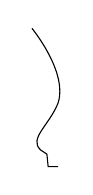
\begin{tikzpicture}[baseline=-2.3em,x=.45em,y=.5em,line width=.4pt]
\draw (0,5)..controls(1.7,3)and(2.6,1)..(2.1,-.4)
 ..controls(1.4,-2)and(-.3,-3)..(.7,-3.8)--(1.2,-4.1)--(1.3,-5)--(2.1,-5);
\end{tikzpicture}\begin{minipage}{.89\linewidth}
se donner
d'avance \(u_{\unsure{i|i-1}}=s_i(w)\), \inserted{\(v_{\unsure{i|i-1}}=\)}\(t_i(w)\),
\inserted{de \(F_{i-1}\)} soumis aux seules conditions \deleted{de} que
\(f(u_{\unsure{i|1}})=u'_i\), \inserted{\(\unsure{\text{resp}}\)}
\(g(v_i)=v'_i\)
et, \deleted{de} plus, si \(i-1\geq1\) i.e \(i\geq2\), \deleted{que}
\(s(u)=s(v),\ t(u)=t(v)\)
\end{minipage}

(NB on n'exige pas que \(\unsure{f|g}(u)=u'\))
\end{minipage}
\end{flushright}

\[
\begin{aligned}
\unsure{\Xi|E}_0\quad\text{\textcircled{\(\unsure{\mathrm b)|\mathrm a)}\)}}\quad&
\forall s'\in F'_0,\quad \exists s\in\mathbb F_0,\ u\in F'_1,\quad
f_0(s)\xrightarrow{u}s'\\[-.1em]
&\hspace{4em}\deleted{\pi_0(f)\ \text{surj}}\quad
-\pi_0(f)\ \text{\uuline{\unsure{surj}}}\\
\mathrm b)\quad&
\forall s,t\in F_0,\quad
\underset{\substack{\rotatebox{-90}{\(\in\)}\\F'_1}}{u'}:f_0(s)\longrightarrow f_0(t),\\
&\exists u\in\mathbb F_1,\quad u:s\mathbin{-}t\qquad\pi_0(f)\ \text{inj.}
\end{aligned}
\]

\[
\begin{aligned}
\Xi_1\quad\text{\textcircled{\(\mathrm b')\)}}\quad&
\forall s,t\in F_0,\quad
\underset{\substack{\rotatebox{-90}{\(\in\)}\\F'_1}}{u'}:
 f_0(s)\mathbin{-} f_0(t),\\
&\exists u\in F_1,\quad u:s\mathbin{-}t,\quad
 f(u)\xrightarrow[\smash{\raisebox{1.1ex}{\(\sim\)}}]{\ell}u'\\
&\deleted{\unsure{w|u|\exists w}\in F_2}\\
&\pi_0(f)\ \text{inj. et }\text{\uuline{\(\pi_1(f)\) surj}}
\end{aligned}
\]
% The wavy mark is superposed on the rightward shaft, not a separate line below.

\[
\begin{aligned}
\mathrm c)\quad&
\deleted{\forall s,t\in\mathbb F_0,}\ u,v\in\unsure{\mathbb F|F}_1\quad
\begin{gathered}s_i(u)=s_1(v),\\[-.2em] t_1(u)=t_1(v)\end{gathered},\\
&\text{et }\underset{\substack{\rotatebox{-90}{\(\in\)}\\F'_2}}{w'}:
 f(u)\longrightarrow f(v),\quad
 \exists\underset{\substack{\rotatebox{-90}{\(\in\)}\\F_2}}{w}:
 \deleted{\unsure{f|f_1}}u\mathbin{-}v\\
&\pi_{\unsure{f|1}}(f)\ \text{inj.}
\end{aligned}
\]
\figure{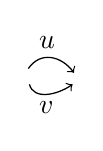
\begin{tikzpicture}[x=1em,y=1em,line width=.45pt]
\draw[->] (0,.45)..controls(.45,1.1)and(1.2,.9)..(1.65,.3);
\draw[->] (.04,-.12)..controls(.2,-.7)and(1.05,-.5)..(1.6,-.12);
\node at (.68,1.38) {$u$};\node at (.65,-.96) {$v$};
\end{tikzpicture}}
% The two curves have visibly separate starts and separate right-hand tips.

\[
\begin{aligned}
E_2\quad\text{\textcircled{\(\mathrm c'\)}}\quad&
\forall(u,v)\in\mathbb F_1,\quad
\begin{gathered}s_1(u)=s_1(v)\\[-.2em] t_1(u)\mathbin{-}t_1(v)\end{gathered}
\quad\text{et }\underset{\substack{\rotatebox{-90}{\(\in\)}\\F'_2}}{w'}:
 f(u)\mathbin{-}f(v),\\
&\exists\underset{\substack{\rotatebox{-90}{\(\in\)}\\F_2}}{w}:u\longrightarrow v\
 \underline{\deleted{\unsure{et|f}}}\ \text{tel que}\\
&w'\sim f(w)
\end{aligned}
\]
% The low horizontal stroke under the cancellation is reproduced as a rule;
% this does not assert that the author intended emphasis.
\figure{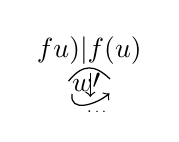
\begin{tikzpicture}[x=1em,y=1em,line width=.45pt]
\node at (.75,1.6) {$\unsure{fu)|f(u)}$};
\draw (0,.5)..controls(.53,1.15)and(.95,1.1)..(1.5,.58);
\draw[->] (.13,.04)..controls(.02,-.65)and(1.0,-.35)..(1.48,.06);
\draw[->] (.79,.8)--(.79,-.07);
\node at (.5,.35) {$w$};\node at (1.01,.5) {$\prime$};
\fill (.75,-.58) circle (.035);\fill (1.03,-.59) circle (.028);\fill (1.28,-.59) circle (.028);
\end{tikzpicture}}
% Upper curve has no discernible head; lower curve has a small rightward head.
% The downward shaft lies between w and its prime; three detached dots are below.

\figure{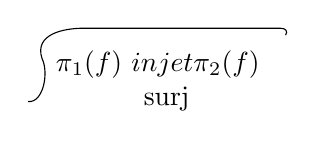
\begin{tikzpicture}[x=1em,y=1em,line width=.4pt]
\node[anchor=west] at (.65,0) {$\pi_1(f)\ \text{inj et }\pi_2(f)$};
\node at (5,-1.25) {surj};
\draw (0,-1.35)..controls(.55,-1.4)and(.75,-.3)..(.5,.2)
 ..controls(.2,1.1)and(1.3,1.3)..(2,1.3)--(9.1,1.3)
 ..controls(9.3,1.3)and(9.4,1.2)..(9.3,1.05);
\end{tikzpicture}}
% The final note has a long curved top-and-left boundary, not a central overbrace.
% archive sheet number: 4
